\section{Ejercicio 2: El Imperio contraataca}

    % Describir detalladamente el problema a resolver dando ejemplos del mismo y sus soluciones.
    \subsection{Descripción del problema}

    \begin{figure}[ht]
        \begin{center}
            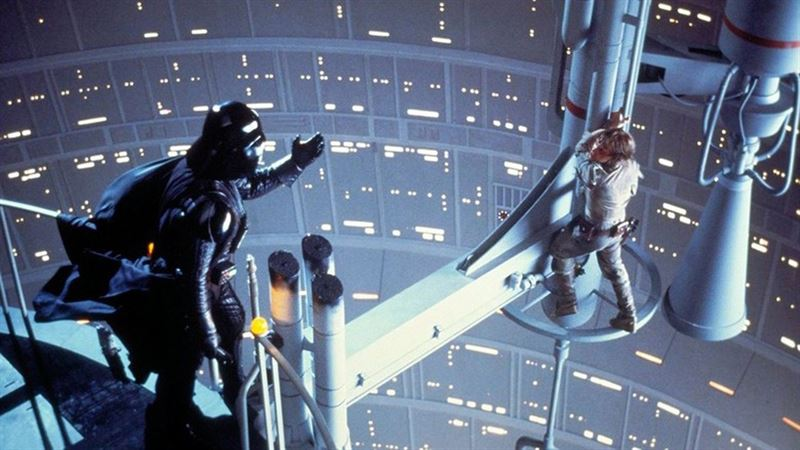
\includegraphics[width=10cm]{imagenes/el_imperio_contraataca.jpg}
            \caption{¡Prestame atención a mí, soy tu padre!}
        \end{center}
    \end{figure}

    Luke debe informarle a todos sus aliados para que estén al tanto del contraataque del Imperio. Parte del planeta Hoth, conocido como planeta 0, y quiere que la noticia llegue a todos los planetas.

    En cada planeta hay infinitos halcones milenarios. Los halcones milenarios consumen una determinada de combustible cada un millón de kilómetros.

    Una vez que un halcón milenario llega a un planeta, de éste pueden salir cualquier cantidad de halcones para seguir advirtiendo a los rebeldes de otros planetas.

    Los halcones milenarios no pueden viajar por cualquier lado, solo por determinadas rutas espaciales. Cada ruta conecta exactamente dos planetas, y recorrer cada ruta consume una determinada cantidad de combustible. Además, se sabe que existe al menos una forma de llegar desde cualquier planeta a cualquier otro a través de rutas espaciales.

    Se pide encontrar cuál es la mínima cantidad de combustible necesaria para entregar el mensaje en todos los planetas. Además, se debe indicar de qué planeta proviene la nave que entrega el mensaje, para cada planeta excepto el 0.

    Se pide que el algoritmo tenga una complejidad temporal $\ord(M$ log $M)$. \\

    \textbf{Formato de entrada}: La primera línea consta de un entero positivo \texttt{N}, que indica la cantidad de planetas, y un entero positivo M, que indica la cantidad de rutas espaciales. A continuación de esta línea siguen \texttt{M} líneas con enteros \texttt{Ai}, \texttt{Bi} y \texttt{Li}, siendo \texttt{Ai} y \texttt{Bi} los extremos de la ruta y \texttt{Li} la cantidad de litros que se gastan al recorrer esa ruta ($0 \leq \mathtt{Ai} \neq \mathtt{Bi} \leq N-1$). La entrada contará con el siguiente formato:

    \begin{verbatim}
    N M
    A0 B0 L0 
    A1 B1 L1 
    ...
    AM-1 BM-1 LM-1
    \end{verbatim}

    \textbf{Formato de salida}: La primera línea debe contener la cantidad mínima de litros \texttt{L} necesarios para informar a toda la alianza sobre esta noticia, seguida de $N-1$ líneas que indican desde qué planeta se viaja para informar de la situación a cada planeta (el vecino inmediato desde el cual se viaja). El formato debe ser el siguiente:
    
    \begin{verbatim}
    L
    I1
    I2
    ...
    IN-1
    \end{verbatim}

    indicando que al planeta \texttt{i} se le informa de la situación con una nave que parte del planeta \texttt{Ii}.

    A continuación se incluyen, a modo de ejemplo, una posible entrada y una
    salida correcta para la misma:

    \begin{tabular}{ll}
    \textbf{Entrada} & \textbf{Salida} \\
    \texttt{4 4}     & \texttt{4}      \\
    \texttt{0 1 1}   & \texttt{0}      \\
    \texttt{1 2 2}   & \texttt{1}      \\
    \texttt{1 3 5}   & \texttt{2}      \\
    \texttt{2 3 1}   &                 \\
    \end{tabular}

    Es importante observar que pueden haber más de una salida distinta válida.

    % Explicar de forma clara, sencilla, estructurada y concisa, las ideas
    % desarrolladas para la resolución del problema. Utilizar pseudocódigo y
    % lenguaje coloquial (no código fuente). Justificar por qué el
    % procedimiento resuelve efectivamente el problema.
    \subsection{Solución propuesta}

    El hecho de que los planetas se encontraran unidos mediante rutas, y que
    cada una de ellas conectara exactamente dos planetas, permitió encarar la
    resolución del problema modelando el sistema planetario mediante un
    grafo, donde cada planeta es un vértice y cada ruta es un eje.

    Para representar los distintos costos de utilizar una u otra ruta
    espacial, se consideró un grafo ponderado, utilizando como peso de cada
    eje la cantidad de combustible que cuesta recorrer la ruta
    correspondiente. Por otra parte, el hecho de que siempre exista forma de
    viajar entre dos planetas equivale a decir que el grafo es conexo.

    Sea $G$ el grafo cuyo conjunto de vértices son los planetas y su conjunto
    de aristas, las rutas espaciales. Bajo este modelo, el problema que busca
    resolverse es hallar un subgrafo $T$ de $G$, de forma tal que:
    \begin{itemize}
        \item Todos los nodos de $G$ sean nodos de $T$.
        \item Llamando $v_0 \in V(G)$ al planeta Hoth, exista en $T$ un camino
        entre $v_0$ y cualquier otro planeta. Dado que $T$ es un grafo no
        dirigido, esto equivale a pedir que $T$ sea conexo.
        \item La suma de los pesos de todos los ejes $T$ sea mínima con
        respecto a todos los subgrafos de $G$ que cumplen los dos puntos
        anteriores.
    \end{itemize}


    \begin{lema}
    Todo subgrafo $T \subseteq G$ que cumpla con los tres puntos anteriores
    es un árbol generador mínimo de $G$.
    \end{lema}
    \begin{proof}

    \end{proof}

    % Deducir una cota de complejidad temporal del algoritmo propuesto (en
    % función de los parámetros que se consideren correctos) y justificar por
    % qué el algoritmo la cumple. Utilizar el modelo uniforme.
    \subsection{Complejidad teórica}

    % Realizar experimentación para medir la performance, usando un conjunto
    % de casos de test que permitan observar los tiempos de ejecución en
    % función de los parámetros de entrada, tanto para instancias aleatorias
    % (detallando cómo fueron generadas) como para instancias particulares
    % (peor/mejor caso, por ejemplo). Presentar en forma gráfica una
    % comparación entre los tiempos medidos y la complejidad teórica y extraer
    % conclusiones.
    \subsection{Experimentación}

    % Ejemplo de gráfico para reutilizar:
    % \begin{figure}[H]
    %     \centering
    %     \caption{}
    %     \label{fig:exp1:tiempo_base}
    %     \begin{tikzpicture}
    %         \begin{axis}[
    %                 title={},
    %                 xlabel={Tamaño de entrada ($N$)},
    %                 ylabel={Tiempo de ejecución (nanosegundos)},
    %                 scaled x ticks=false,
    %                 scaled y ticks=false,
    %                 enlargelimits=0.05,
    %                 width=0.5\textwidth,
    %                 height=0.5\textwidth,
    %                 legend pos=south east,
    %                 legend cell align=left,
    %                 xmin=1
    %             ]
    %             \addplot[color=black] table[x index=0,y index=1]{../exp/kaioKenOutput};
    %             \addplot[color=red] table[x index=0, y expr={x*ln(x)*\constante}]{../exp/kaioKenOutput};
    %             \legend{$T$, $c*N*log(N)$}
    %         \end{axis}
    %     \end{tikzpicture}
    % \end{figure}
